%%%%%%%%%%%%%%%%%%%%%%%%%%%%%%%%%%%%%%%%%%%%%%%%%%%%%%%%%%%%
%%% ELIFE ARTICLE TEMPLATE
%%%%%%%%%%%%%%%%%%%%%%%%%%%%%%%%%%%%%%%%%%%%%%%%%%%%%%%%%%%%
%%% PREAMBLE 
\documentclass[9pt,lineno,final]{elife}
% Use the onehalfspacing option for 1.5 line spacing
% Use the doublespacing option for 2.0 line spacing
% Please note that these options may affect formatting.
% Additionally, the use of the \newcommand function should be limited.


\usepackage{lipsum} % Required to insert dummy text
\usepackage[version=4]{mhchem}
\usepackage{siunitx}
\usepackage[color=green!30, textsize=small]{todonotes}
\usepackage{float}
\usepackage{graphicx}
\usepackage{grffile}

\usepackage{algorithm2e}
\usepackage{cleveref} % use \cref or \Cref to refer to labeled elements for automatically referring to the right type of entity, with the right capital letter and/or abbreviation rules
\usepackage[subpreambles=true]{standalone}

\DeclareSIUnit\Molar{M}

\newcommand{\pH}{\mathrm{pH}}
\newcommand{\pKa}{\mathrm{pKa}}

%%%%%%%%%%%%%%%%%%%%%%%%%%%%%%%%%%%%%%%%%%%%%%%%%%%%%%%%%%%%
%%% ARTICLE SETUP
%%%%%%%%%%%%%%%%%%%%%%%%%%%%%%%%%%%%%%%%%%%%%%%%%%%%%%%%%%%%
\title{SAMPL6 pKa reference calculations using Epik and Jaguar}

\author[1,2]{Ari\"{e}n S. Rustenburg}
\author[1]{Mehtap Isik}
\author[1,2]{Patrick B. Grinaway}
\author[1,3]{Andrea Rizzi}
%\author[4]{Art Bochevarov}
%\author[4]{John Shelley}
\author[5]{Marilyn R Gunner}
\author[1*]{John D. Chodera}

\affil[1]{Computational and Systems Biology Program, Sloan Kettering Institute, Memorial Sloan Kettering Cancer Center, New York, NY 10065}
\affil[2]{Graduate Program in Physiology, Biophysics, and Systems Biology, Weill Cornell Medical College, New York, NY 10065}
\affil[3]{Tri-Institutional Training Program in Computational Biology and Medicine, New York, NY 10065}
\affil[4]{Schrödinger LLC, New York, NY 10036}
\affil[5]{Department of Physics, City College of New York, New York, NY 10031}
\corr{john.chodera@choderalab.org}{JDC}

%\presentadd[\authfn{3}]{Schr\"{o}dinger, New York, NY 10036}

%\contrib[\authfn{1}]{These authors contributed equally to this work}
%\contrib[\authfn{2}]{These authors also contributed equally to this work}

%%%%%%%%%%%%%%%%%%%%%%%%%%%%%%%%%%%%%%%%%%%%%%%%%%%%%%%%%%%%
%%% ARTICLE START
%%%%%%%%%%%%%%%%%%%%%%%%%%%%%%%%%%%%%%%%%%%%%%%%%%%%%%%%%%%%

\begin{document}

\maketitle

\section{NOTES: Objectives for this manuscript}
\todo[inline]{track down type II artifacts, and dont use type I labels, use epik scan, sequential, et cetera}
\begin{itemize}
	\item Provide a baseline for the expectation of performance of empirical models (Epik) and DFT models (Jaguar) on kinase inhibitor-like molecules and molecular fragments; draw comparisons to earlier benchmarks for these tools
	\item Describe basic concepts, along with strengths and weaknesses of each approach (Epik and Jaguar)
	\item Lessons learned for participating in the challenge
	      \begin{itemize}
	      	\item How should we predict macroscopic pKas from microscopic pKas? Explain possibilities and justify choice
	      	      \begin{itemize}
	      	      	\item Sequential titration (Epik)
	      	      	\item <n protons>/charge vs pH inflection points: Matches electrochemical titration, but not UV-metric
	      	      	\item Is there a way to predict what UV-metric would observe from populations vs pH?
	      	      \end{itemize}
	      \end{itemize}
	\item For microscopic pKa prediction: Epik may enumerate a different set of microstates than other tools (we proposed these as newly labeled states)
	\item Epik does not return state populations below a certain threshold, so we could not consider states proposed by SAMPL6 [Check this]
	\item For worst predicted compounds, provide an explanation as to why the methods may perform poorly (descriptors?) [ may not have enough data points to draw conclusion]
	      
\end{itemize}

\section{Figures and Tables}

\begin{figure}[H]
	\centering
	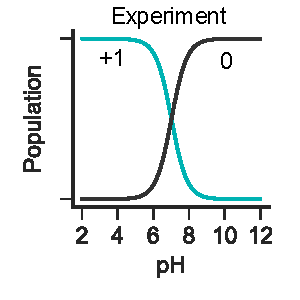
\includegraphics[width=0.33\textwidth]{Reports/Experiment-populations-SM03-titled.pdf}
	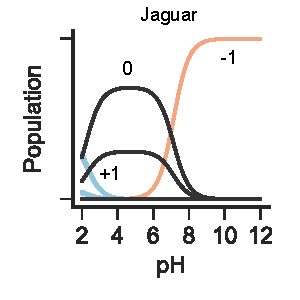
\includegraphics[width=0.33\textwidth]{Reports/Jaguar-pKa-populations-SM03-titled.pdf}
	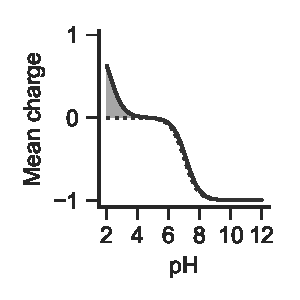
\includegraphics[width=0.33\textwidth]{Reports/Jaguar-pKa-virtual-titration-SM03.pdf}\\
	Charge \\
	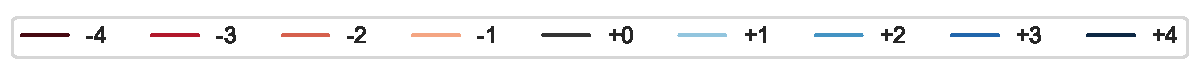
\includegraphics[width=0.66\textwidth, trim={2cm 0 2cm 0},clip]{Reports/overview-charge-legend-SM03.pdf}
		\caption{{\bf Comparing UV experiments for SM03 to microscopic pKa Jaguar predictions}. This example shows how the UV experimental populations (left) for macrostates molecule SM03 as a function of the pH can be compared to Jaguar predictions. Jaguar was used to predict microscopic pKas (denoted as Type I predictions in SAMPL6), which can be used to derive relative microstate populations (middle). In the UV experiment, charge reflects the number of protonations, since absolute charge information is unknown. The charge combined with populations produces a macroscopic titration curve (right), with the prediction as a solid, and the experiment as a dashed line. The area between the curves (gray) is calculated after correcting for an integer offset in charges.
	\label{fig:jaguar-prediction}}
	\todo[inline]{ASR: Add number of area to plot}
\end{figure}


\begin{figure}[H]
	\centering
	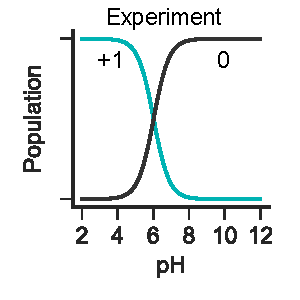
\includegraphics[width=0.33\textwidth]{Reports/Experiment-populations-SM04-titled.pdf}
	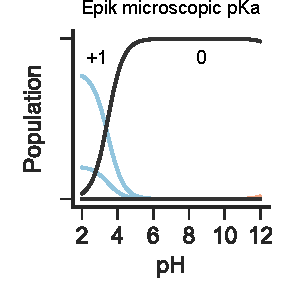
\includegraphics[width=0.33\textwidth]{Reports/Epik-micropka-populations-SM04-titled.pdf}
	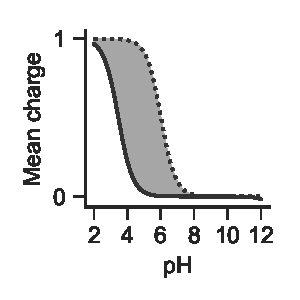
\includegraphics[width=0.33\textwidth]{Reports/Epik-micropka-virtual-titration-SM04.pdf}\\
	Charge \\
	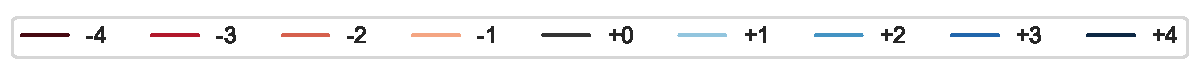
\includegraphics[width=0.66\textwidth, trim={2cm 0 2cm 0},clip]{Reports/overview-charge-legend-SM03.pdf}
		\caption{{\bf Comparing UV experiments for SM04 to Epik microscopic pKa predictions} .This example shows how the UV experimental populations (left) for macrostates molecule SM04 as a function of the pH can be used to compare to microscopic pKa Epik predictions. Epik was used to predict microscopic pKas (denoted as Type I predictions in SAMPL6), which can be used to derive relative microstate populations (middle). In the UV experiment, charge reflects the number of protonations, since absolute charge information is unknown. The charge combined with populations produces a macroscopic titration curve (right), with the prediction as a solid, and the experiment as a dashed line. The area between the curves (gray) is calculated after correcting for an integer offset in charges.  
	\label{fig:epiki-prediction}}
\end{figure}

\begin{figure}[H]
	\centering
	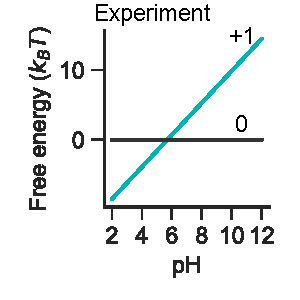
\includegraphics[width=0.33\textwidth]{Reports/Experiment-free-energy-SM20-titled.pdf}
	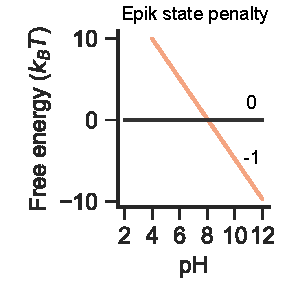
\includegraphics[width=0.33\textwidth]{Reports/Epik-free-energy-free-energy-SM20-titled}
	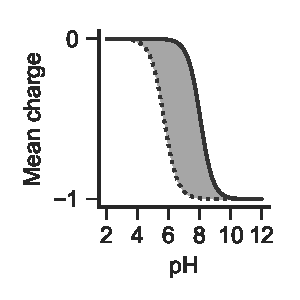
\includegraphics[width=0.33\textwidth]{Reports/Epik-free-energy-virtual-titration-SM20.pdf}\\
	Charge \\
	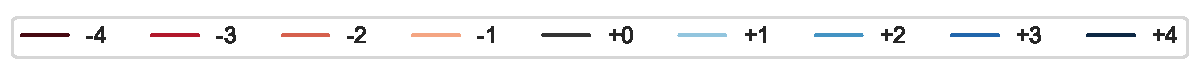
\includegraphics[width=0.66\textwidth, trim={2cm 0 2cm 0},clip]{Reports/overview-charge-legend-SM03.pdf}
		\caption{{\bf Comparing UV experiments for SM20 to Epik microscopic free energy predictions} .This example shows how the UV experimental free energy (left) for macrostates molecule SM20 as a function of the pH can be compared to microscopic free energy Epik predictions. Epik was used to predict microscopic free energy (denoted as Type II predictions in SAMPL6) (middle). In the UV experiment, charge reflects the number of protonations, since absolute charge information is unknown. The charge combined with free energies produces a macroscopic titration curve (right), with the prediction as a solid, and the experiment as a dashed line. The area between the curves (gray) is calculated after correcting for an integer offset in charges.  
	\label{fig:epikii-prediction}}
\end{figure}


\begin{figure}[H]
	\centering
	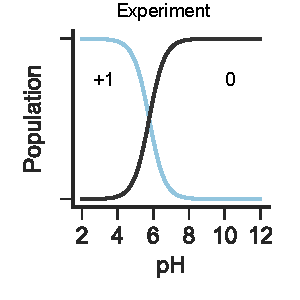
\includegraphics[width=0.33\textwidth]{Reports/Experiment-populations-SM13-titled.pdf}
	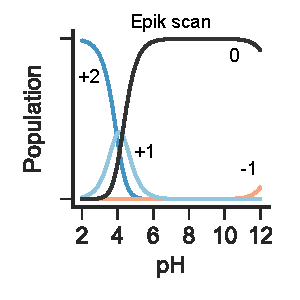
\includegraphics[width=0.33\textwidth]{Reports/Epik-scan-populations-SM13-titled.pdf}
	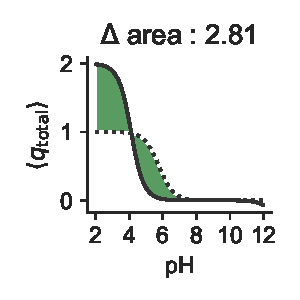
\includegraphics[width=0.33\textwidth]{Reports/Epik-scan-virtual-titration-SM13.pdf}\\
	Charge \\
	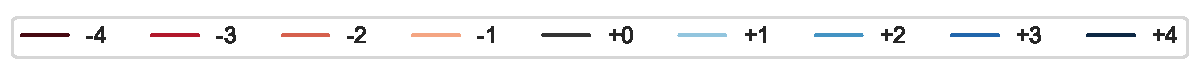
\includegraphics[width=0.66\textwidth, trim={2cm 0 2cm 0},clip]{Reports/overview-charge-legend-SM03.pdf}
		\caption{{\bf Comparing UV experiments for SM13 to Epik macroscopic pKa predictions} .This example shows how the UV experimental populations (left) for macrostates molecule SM13 as a function of the pH can be compared to sequential pKa Epik predictions. Epik scan mode was used to predict macroscopic pKa values (denoted as Type III predictions in SAMPL6), which can be translated into relative macrostate populations (middle). In the UV experiment, charge reflects the number of protonations, since absolute charge information is unknown. The charge combined with populations produces a macroscopic titration curve (right), with the prediction as a solid, and the experiment as a dashed line. The area between the curves (gray) is calculated after correcting for an integer offset in charges.    
	\label{fig:epikiii-prediction}}
\end{figure}

\begin{table}[H]
	\centering
	\caption{Overall performance of each method using either the closest pKa matching, Hungarian pKa matching,  and the area between the experimental and predicted macroscopic charge titration curve}
	\label{tab:overview-performance}
	\begin{tabular}{c|ccc|ccc|c}
		& \multicolumn{3}{c|}{Closest} & \multicolumn{3}{c|}{Hungarian} & Titration curve \\ \cline{2-8} 
		                & RMSE & MAE & $R^2$ & RMSE & MAE & $R^2$ & $\Delta $ area \\ \hline
		Epik sequential &      &     &       &      &     &       &           \\
		Epik micropka   &      &     &       &      &     &       &           \\
		Jaguar micropKa &      &     &       &      &     &       &           
	\end{tabular}
\end{table}
    

\begin{figure}[H]
\centering
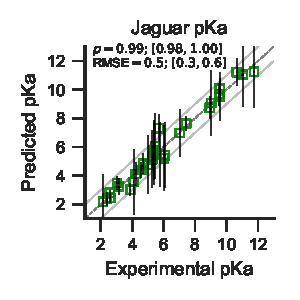
\includegraphics[]{closest_pka_jaguar.pdf}
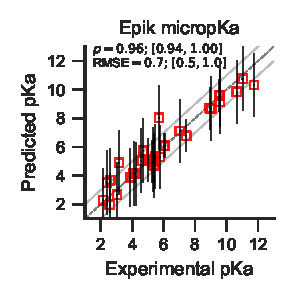
\includegraphics[]{closest_pka_epik_micropka.pdf}
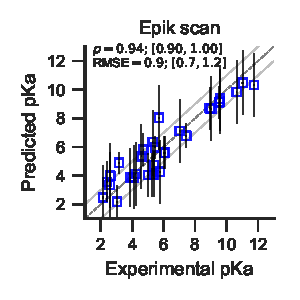
\includegraphics[]{closest_pka_epik_scan.pdf}
\caption{{\bf Comparison of computed pKa values to experimental macroscopic pKa values.} {\it Left:} Microscopic pKa values for Jaguar were matched ot the experimental dataset using \cref{alg:closest}. An alternative alignment of pKa values using the Hungarian algorithm (\cref{alg:hungarian}) is available as a supplementary figure.
{\it Middle:} Microscopic pKa values for Epik were matched ot the experimental dataset using \cref{alg:closest}. An alternative alignment of pKa values using the Hungarian algorithm (\cref{alg:hungarian}) is available as a supplementary figure.
{\it Right:} Macroscopic pKa values for Jaguar were matched ot the experimental dataset using \cref{alg:closest}. An alternative alignment of pKa values using the Hungarian algorithm (\cref{alg:hungarian}) is available as a supplementary figure. \label{correlation-closest}}


\end{figure}
    

\begin{figure}[H]
	\centering
	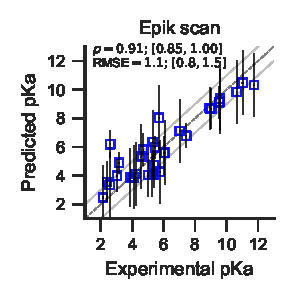
\includegraphics[scale=1.0]{aligned_pka_epik_scan.pdf}	
	\caption{{\bf Epik macroscopic pKa values compared to macroscopic experimental pKa values, sequentially matching pKa values}
		Comparison of the Epik sequential scan with entire experimental data set is shown, allowing only sequential pKa values to match experiment.\label{fig:correlation-sequential}}
\end{figure}
    
    
\begin{table}[H]
	\todo[inline]{Add columns for the other two algorithms}
	\centering
	\caption{{\bf Macroscopic pKas computed via Epik's sequential scan procedure.}
		Experimental and computed pKa values matched using \cref{alg:closest}.}
	\small
	\label{tab:molecule-macro}
	\rowcolors{2}{gray!25}{white}
	\begin{tabular}{lrr}
		\toprule
		{\bf Molecule} & {\bf Experiment $\pm$ SEM} & {\bf Epik closest $\pm$ SEM} \\
		\midrule
		SM01           & 9.53$\pm$0.01            & 9$\pm$1                  \\
		SM02           & 5.03$\pm$0.01            & 4$\pm$2                  \\
		SM03           & 7.02$\pm$0.01            & 7$\pm$2                  \\
		SM04           & 6.02$\pm$0.01            & 6$\pm$1                  \\
		SM05           & 4.59$\pm$0.01            & 5$\pm$2                  \\
		SM06           & 3.03$\pm$0.04              & 2$\pm$1                  \\
		SM06           & 11.74$\pm$0.01           & 10$\pm$2                 \\
		SM07           & 6.08$\pm$0.01            & 6$\pm$1                  \\
		SM08           & 4.22$\pm$0.01            & 4$\pm$2                  \\
		SM09           & 5.37$\pm$0.01            & 4$\pm$2                  \\
		SM10           & 9.02$\pm$0.01            & 9$\pm$2                  \\
		SM11           & 3.89$\pm$0.01            & 4$\pm$2                 \\
		SM12           & 5.28$\pm$0.01            & 4$\pm$2                  \\
		SM13           & 5.77$\pm$0.01            & 4$\pm$2                  \\
		SM14           & 2.58$\pm$0.01           & 3$\pm$2                  \\
		SM14           & 5.30$\pm$0.01            & 6$\pm$2                  \\
		SM15           & 8.94$\pm$0.01            & 9$\pm$1                  \\
		SM15           & 4.70$\pm$0.01            & 6$\pm$1                  \\
		SM16           & 5.37$\pm$0.01            & 4.7$\pm$0.9                  \\
		SM16           & 10.65$\pm$0.01           &  10$\pm$2                  \\
		SM17           & 3.16$\pm$0.01            & 4.9$\pm$0.7                  \\
		SM18           & 9.58$\pm$0.03            & 9$\pm$2                  \\
		SM18           & 2.15$\pm$0.02            & 2.5$\pm$2                  \\
		SM18           & 11.02$\pm$0.04             & 11$\pm$2                 \\
		SM19           & 9.56$\pm$0.02            & 9$\pm$2                  \\
		SM20           & 5.70$\pm$0.03            & 8$\pm$2                  \\
		SM21           & 4.10$\pm$0.01            & 4$\pm$2                  \\
		SM22           & 7.43$\pm$0.01            & 6.8$\pm$0.9                  \\
		SM22           & 2.40$\pm$0.02            & 4$\pm$1                  \\
		SM23           & 5.45$\pm$0.01            & 6.0$\pm$0.8                  \\
		SM24           & 2.60$\pm$0.01            & 4$\pm$2                  \\
		\bottomrule
	\end{tabular}
	    
\end{table}
    
\begin{table}[H]
	\todo[inline]{Add table for the Hungarian algorithm to SI.}
	\centering
	\caption{{\bf Microscopic pKa per molecule for each method as matched by \cref{alg:closest}, compared to experiment.}}
	\label{tab:molecule-macro}
	\begin{tabular}{l|llllll}
		           & \multicolumn{1}{c}{Experimental pKa} & \multicolumn{1}{c}{Epik pKa} & \multicolumn{1}{c}{Epik pKa uncertainty} & \multicolumn{1}{c}{Epik error} & \multicolumn{1}{c}{Jaguar pKa} & \multicolumn{1}{c}{Jaguar error} \\ \hline
		SM01 pKa1  &                                      &                              &                                          &                                &                                &                                  \\
		SM01 pKa2  &                                      &                              &                                          &                                &                                &                                  \\
		SM02 pKa 1 &                                      &                              &                                          &                                &                                &                                  \\
		SM03 pKa 1 &                                      &                              &                                          &                                &                                &                                  
	\end{tabular}
\end{table}
    
    
\begin{figure}[H]
	\centering
	\todo[inline]{ASR: Find a good place to put the legen, find source of free energy/ state penalty discrepancy artifacts}
	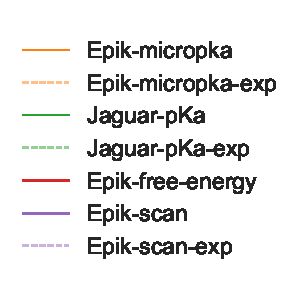
\includegraphics[]{Reports/overview-legend-SM01.pdf}	\\
	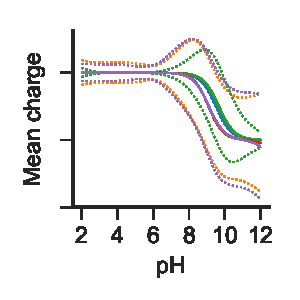
\includegraphics[width=0.33\textwidth]{Reports/overview-virtual-titration-SM01.pdf}
	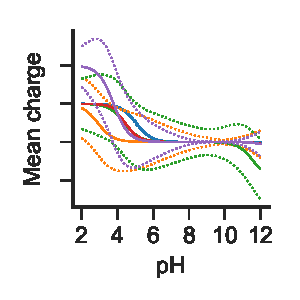
\includegraphics[width=0.33\textwidth]{Reports/overview-virtual-titration-SM02.pdf}
	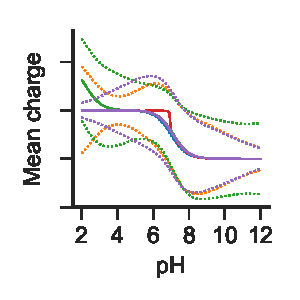
\includegraphics[width=0.33\textwidth]{Reports/overview-virtual-titration-SM03.pdf}	 \\
		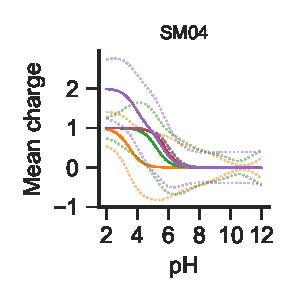
\includegraphics[width=0.33\textwidth]{Reports/overview-virtual-titration-SM04.pdf}
	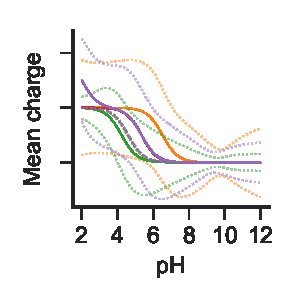
\includegraphics[width=0.33\textwidth]{Reports/overview-virtual-titration-SM05.pdf}
	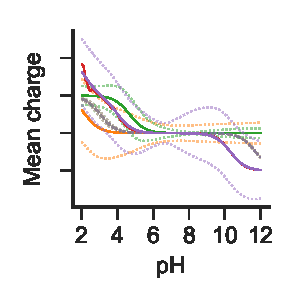
\includegraphics[width=0.33\textwidth]{Reports/overview-virtual-titration-SM06.pdf}	 \\
		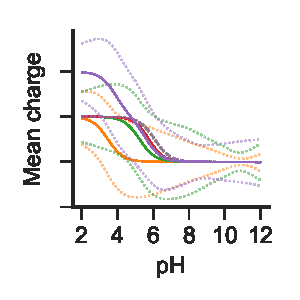
\includegraphics[width=0.33\textwidth]{Reports/overview-virtual-titration-SM07.pdf}
	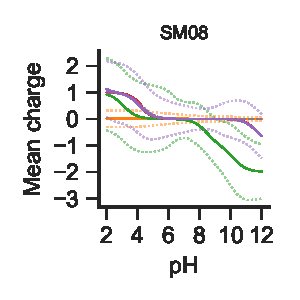
\includegraphics[width=0.33\textwidth]{Reports/overview-virtual-titration-SM08.pdf}
	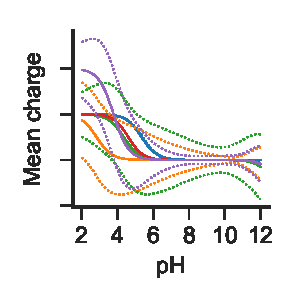
\includegraphics[width=0.33\textwidth]{Reports/overview-virtual-titration-SM09.pdf}	 \\
	\caption{{\bf Bootstrap titration curves for each method compared to experiment for molecules SM01-SM09.} The titration curve for each method is shown as a solid line, and 96 \% confidence intervals from bootstrap have been shown as dotted lines. A numerical comparison to experiment is presented in \cref{tab:titration-curves}.
	\label{fig:charge-curves1}}
	\end{figure}
	
	
\begin{figure}[H]	
	\centering
	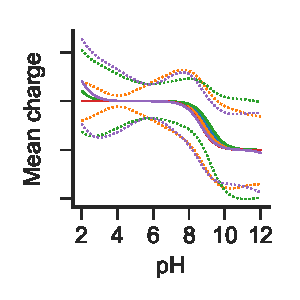
\includegraphics[width=0.33\textwidth]{Reports/overview-virtual-titration-SM10.pdf}
	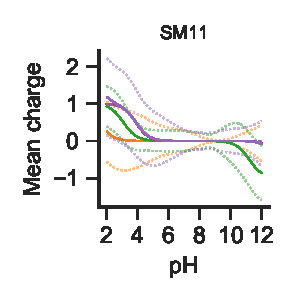
\includegraphics[width=0.33\textwidth]{Reports/overview-virtual-titration-SM11.pdf}
	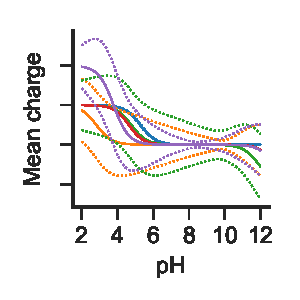
\includegraphics[width=0.33\textwidth]{Reports/overview-virtual-titration-SM12.pdf}	 \\
	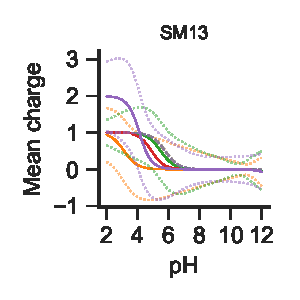
\includegraphics[width=0.33\textwidth]{Reports/overview-virtual-titration-SM13.pdf}
	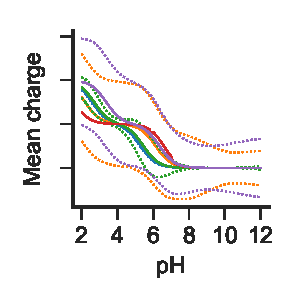
\includegraphics[width=0.33\textwidth]{Reports/overview-virtual-titration-SM14.pdf}
	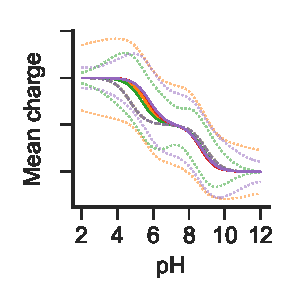
\includegraphics[width=0.33\textwidth]{Reports/overview-virtual-titration-SM15.pdf}	 \\
	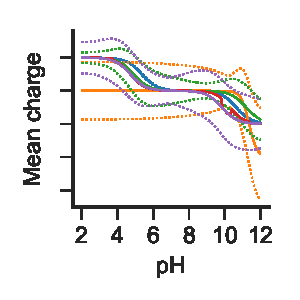
\includegraphics[width=0.33\textwidth]{Reports/overview-virtual-titration-SM16.pdf}
	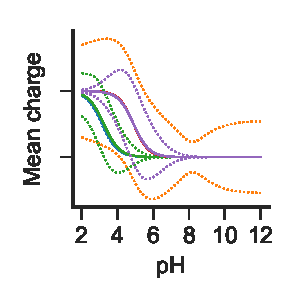
\includegraphics[width=0.33\textwidth]{Reports/overview-virtual-titration-SM17.pdf}
	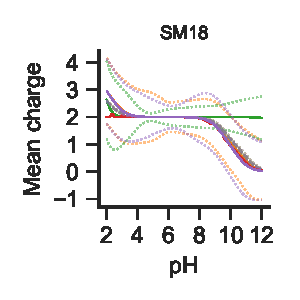
\includegraphics[width=0.33\textwidth]{Reports/overview-virtual-titration-SM18.pdf}	 \\
%		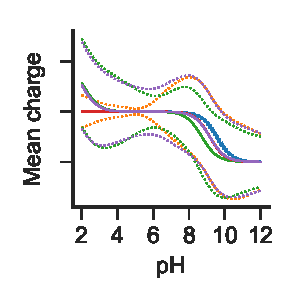
\includegraphics[width=0.33\textwidth]{Reports/overview-virtual-titration-SM19.pdf}
%	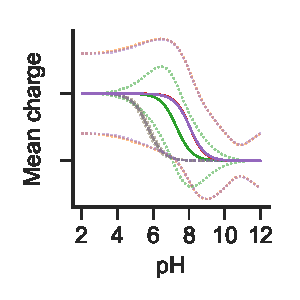
\includegraphics[width=0.33\textwidth]{Reports/overview-virtual-titration-SM20.pdf}
%	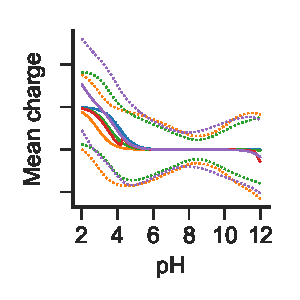
\includegraphics[width=0.33\textwidth]{Reports/overview-virtual-titration-SM21.pdf}	 \\
%		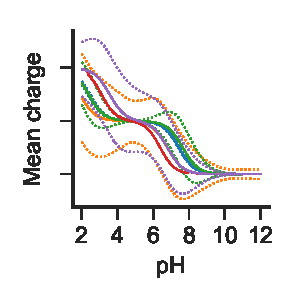
\includegraphics[width=0.33\textwidth]{Reports/overview-virtual-titration-SM22.pdf}
%	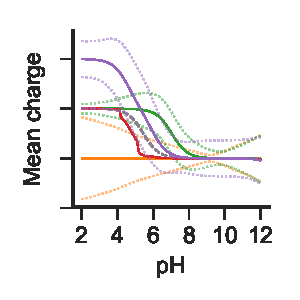
\includegraphics[width=0.33\textwidth]{Reports/overview-virtual-titration-SM23.pdf}
%	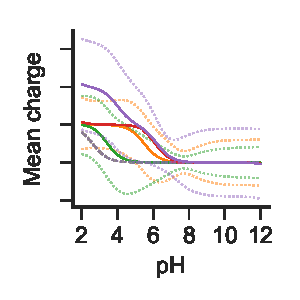
\includegraphics[width=0.33\textwidth]{Reports/overview-virtual-titration-SM24.pdf}	 \\
	\caption{{\bf Bootstrap titration curves for each method compared to experiment for molecules SM10-SM18.} The titration curve for each method is shown as a solid line, and 96 \% confidence intervals from bootstrap have been shown as dotted lines. A numerical comparison to experiment is presented in \cref{tab:titration-curves}.
	\label{fig:charge-curves2}}

\end{figure}
    
 \begin{figure}[H]	
	\centering
	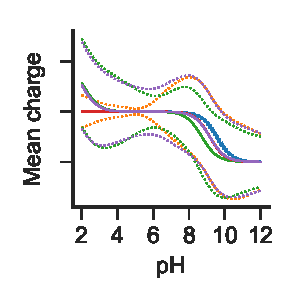
\includegraphics[width=0.33\textwidth]{Reports/overview-virtual-titration-SM19.pdf}
	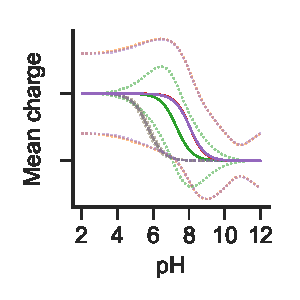
\includegraphics[width=0.33\textwidth]{Reports/overview-virtual-titration-SM20.pdf}
	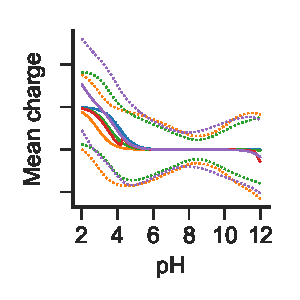
\includegraphics[width=0.33\textwidth]{Reports/overview-virtual-titration-SM21.pdf}	 \\
	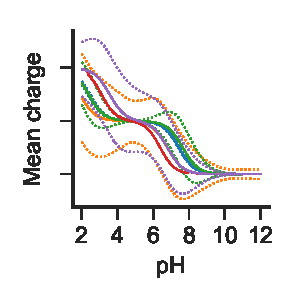
\includegraphics[width=0.33\textwidth]{Reports/overview-virtual-titration-SM22.pdf}
	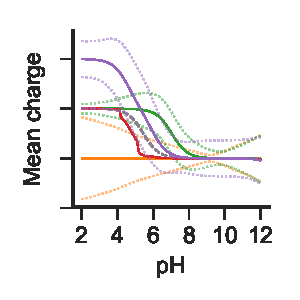
\includegraphics[width=0.33\textwidth]{Reports/overview-virtual-titration-SM23.pdf}
	\includegraphics[width=0.33\textwidth]{Reports/overview-virtual-titration-SM24.pdf}	 \\
	\caption{{\bf Bootstrap titration curves for each method compared to experiment for molecules SM19-SM24.} The titration curve for each method is shown as a solid line, and 96 \% confidence intervals from bootstrap have been shown as dotted lines. A numerical comparison to experiment is presented in \cref{tab:titration-curves}.
	\label{fig:charge-curves3}}

\end{figure}


\begin{table}[H]
	\todo[inline]{ ASR:Need to add new data, and bootstrap error bars.}
	\centering
	\caption{{\bf Difference in area between derived macroscopic charge titration curves ($\Delta$ area ) for each method.} The macroscopic charge curve was constructed for each of the methods, and after alignment with the experimental curve by an integer offset, the area between the curves is reported.}
	\label{tab:titration-curves}
	\rowcolors{2}{gray!25}{white}
	\begin{tabular}{lrrrr}
		\toprule
		Molecule &  Epik microscopic pKa &  Epik microscopic population  &  Epik scan &   Jaguar microscopic pKa \\
		    
		\midrule
		SM01 &       0.43 &        0.44 &         0.46 &         0.15 \\
		SM02 &       2.12 &        0.59 &         1.99 &         1.21 \\
		SM03 &       0.10 &        0.29 &         0.09 &         0.57 \\
		SM04 &       2.55 &        0.26 &         2.20 &         0.81 \\
		SM05 &       1.93 &        0.74 &         1.08 &         0.51 \\
		SM06 &       2.60 &        2.52 &         2.62 &         2.09 \\
		SM07 &       2.61 &        0.32 &         2.25 &         0.84 \\
		SM08 &       1.27 &        0.57 &         0.63 &         5.82 \\
		SM09 &       2.53 &        0.78 &         2.32 &         1.09 \\
		SM10 &       0.17 &        0.34 &         0.62 &         0.28 \\
		SM11 &       1.84 &        0.06 &         0.14 &         1.68 \\
		SM12 &       2.48 &        0.71 &         2.26 &         0.88 \\
		SM13 &       2.64 &        0.88 &         2.80 &         0.30 \\
		SM14 &       1.07 &        1.74 &         1.75 &         0.25 \\
		SM15 &       1.07 &        1.32 &         1.31 &         0.85 \\
		SM16 &       4.36 &        1.10 &         1.44 &         0.97 \\
		SM17 &       1.71 &        1.71 &         1.71 &         0.07 \\
		SM18 &       0.74 &        1.02 &         1.00 &          NaN \\
		SM19 &       0.38 &        0.39 &         0.73 &         1.22 \\
		SM20 &       2.34 &        2.34 &         2.34 &         1.60 \\
		SM21 &       1.26 &        0.70 &         0.55 &         1.68 \\
		SM22 &       0.94 &        1.62 &         1.64 &         0.23 \\
		SM23 &       0.38 &        0.68 &         3.17 &         NaN \\
		SM24 &       0.61 &        3.46 &         5.62 &         NaN \\
		\midrule
		Average &       1.59 &        1.03 &         1.70 &         1.10 \\
		\bottomrule\end{tabular}
		        
		\end{table}
		
	
		
		
		\begin{figure}[H]	
		\centering
		\includegraphics[width=0.33\textwidth]{Images/Molecules/SM03-smarts.png}
		\includegraphics[width=0.33\textwidth]{Images/Molecules/SM18-smarts.png}
		\includegraphics[width=0.33\textwidth]{Images/Molecules/lewis-problem.png}
		\caption{{\bf Problematic lewis structure generated by Epik.}
		Epik generated protonation states with invalid Lewis structure for SM03 and SM18, with a pentavalent nitrogen present in the thiazole/thiadiazole (the protonation pattern displayed on the right). One of these was also present in the set provided as part of SAMPL6  microstates, namely SM03\textunderscore{}micro021. A valid Lewis structure could not be figured out for this protonation state.}
		\label{fig:lewis-structure-SM03-SM18}
		\end{figure}		



      

\todo[inline]{See Images folder for titration curves and free energy images for each category. Will be added to supplementary info later.}

\begin{abstract}
	The goal of the SAMPL6 pKa Challenge was to evaluate the performance of small molecule pKa prediction methods from challenge participants in a blinded fashion on a set of small, drug-like molecules resembling kinase inhibitor fragments.
	%
	To provide a useful point of comparison for blind participant predictions that may use experimental methods still under development, we performed reference benchmark calculations using a popular empirical model (Epik) and quantum chemical approach (Jaguar) from Schrödinger.
	%
	Epik predicts microstate populations and pKas using a Hammett-Taft type model, while Jaguar is a fast DFT quantum chemical method.
	%
	In this work, we discuss how these reference calculations were performed, provide a broad assessment of the performance of the method, and highlight challenges and considerations in predicting pKas to benchmark against experiment macroscopic pKa measurements.
\end{abstract}


\section{Introduction}

Titratable sites are ubiquitous in druglike small molecules.
\todo[inline]{JDC: It would be very useful if we could cite some sort of reference discussing how important protonation states are in small molecule drugs or druglike molecules, but I'm failing to find useful references right now. Alternatively, we could pull pKas from DrugBank \url{https://www.drugbank.ca/releases/latest} or use Epik to make our own plots, like the kinase inhibitor pKa plot we had previously generated.}
%
Large-scale computational surveys suggest that 60\% of all protein-ligand complexes undergo a change in ionization state upon binding~\cite{Aguilar:Biophys.J.:2010}, either due to protonation state changes of the small molecule or the protein (where roughly a third of all protein residues are ionizable~\cite{Jordan:Nature:2005}).
%
More generally, protonation state effects---in which the dominant protonation, charge, or tautomer state shifts upon binding, or a mixture of protonation states are significantly populated in complex or solution---has the potential to cause large modeling errors if these effects are neglected.
%
In the SAMPL5 distribution coefficient (logD) challenge, for example, protonation state effects were determined to be a major contributor to loss in accuracy for the otherwise mundane task of predicting a transfer free energy between aqueous and cyclohexane phases~\cite{Pickard:J.Comput.AidedMol.Des.:2016}.

To isolate the question of how well pKa effects could be modeled---and therefore how accurately the community could address these effects---the SAMPL6 challenge featured a blind pKa prediction component, as an intermediate step to logD predictions in which we provide participants with pKas and later have them predict both pKa and logD~\cite{sampl6-pKa-measurements}.
The SAMPL6 pKa challenge consisted of predicting macroscopic pKas measured by UV-metric titration for a set of small moelcules that resembled kinase inhibitors and their fragments~\cite{sampl6-pKa-measurements}.
As participants in the SAMPL6 pKa challenge were expected to utilize a wide variety of methods still under development, we endeavored to provide a useful baseline reference set of predictions using well-established, widely-deployed, commercially available methods.
We selected both an empirical method (Epik~\cite{Shelley:J.Comput.AidedMol.Des.:2007b}) and quantum chemical method (Jaguar~\cite{Bochevarov:Int.J.QuantumChem.:2013}) from the Schr\"{o}dinger Suite of computational chemistry software, version 20XX-X.

Reference calculations---which were not fully blinded---were performed in a manner that attempted to mimic standard use, using recommended settings for each program, without significantly modifying the input parameters.
As the computation of UV-metric macroscopic pKas from the microscopic pKas predicted by the tools is not necessarily completely straightforward, we considered several alternative possibilities, which we discuss in more detail.
We provide an analysis and broad assessment of the performance of the two methods, and highlight challenges and considerations in predicting pKas to benchmark against experiment.
All analysis tools used to perform this study are available via GitHub at
\url{https://github.com/choderalab/SAMPL6-Reference-pKa-Calculations}

\section{Methods}
\subsection{Epik}
Summary of how Epik works \todo[inline]{Could be filled in by John Shelley?}

\subsection{Jaguar}

Summary of how Jaguar computes pKas  \todo[inline]{Could be filled in by Art Bochevarov?}

\subsection{Microstate predictions}

\subsubsection{Epik: Fast empirical pKa predictions}
\begin{itemize}
	\item were performed between pH 2-12
	\item Reported states with a minimum population of $e^{-10/RT}$
	\item States proposed by SAMPL6 but not predicted by Epik were not considered in analysis.
	      
\end{itemize}


\subsubsection{Jaguar: Ab initio quantum chemical pKa predictions}
\begin{itemize}
	\item Ran using default settings (5 conformations) for each of the pre-enumerated specified microstate pairs.
	\item Input structures were first minimized using MMFF.
	\item Additional minimization was performed for structures for which scf/geopt did not converge
\end{itemize}

\subsection{Predicting macroscopic pKas}

Epik and Jaguar predict microscopic pKas or microstate energies, which must be translated into macroscopic pKas for comparison to experiment.
Several reasonable choices are possible for translating these microscopic properties into macroscopic pKas.

\subsubsection{Sequential titration of dominant species} 

\begin{itemize}
	\item Sequential titration avoids the need to compute the energies of \emph{all} protonation states
	\item Epik can automatically perform a sequential scan (which can also be used in Jaguar with some automation)
	\item For this experiment, we started from the predicted highest-occupancy microstate at pH 7 and went in both directions, returning pKas between 2-12
\end{itemize}

\subsubsection{Virtual electrochemical titration}
\begin{itemize}
	\item Average charge vs pH to match electrochemical titrations, look at the mean signed deviation (MSD) to see whether the charge curve behavior matches
\end{itemize}

\subsubsection{Predicting UV-metric titration}
\begin{itemize}
	\item Actual experiments were UV-metric, where only UV-active transitions are observable
	\item There is potentially a route to predicting UV-active transitions via identifying of microstates that would have different UV spectra, perhaps using SMARTS matches or simple QM absorption spectra calculations?
\end{itemize}

\section{Results}
\begin{itemize}
	\item How much conformation-dependence is there in Jaguar-derived pKas (or state energies)?
	\item Does sequential scan or mean molecular charge provide better agreement with experimental macroscopic pKas? Would it be worthwhile to develop predictive UV-metric models?
	\item Comparison of observed accuracies to previously reported/expected accuracies; expected accuracy on kinase inhibitors derived from this study
	\item How does Epik compare to Jaguar in terms of accuracy and computational cost?
	\item Discussion of outliers
\end{itemize}

\section{Discussion}



\subsection{Overall performance}

Some low probability structures produced by Epik included questionable protonation states of a heterycyclic moiety, present in SM03 and SM18 ( \Cref{fig:lewis-structure-SM03-SM18}). 



Overall performance of Epik and Jaguar based on various metrics (figures/tables)
\subsubsection {Matching of experimental and calculated pKas}


The experiments do not provide any microscopic information on what atom, or microstate a pKa belongs to.
%
Therefore, it is necessary to perform a matching of pKa values between experiment and predicted pKa values.
%
There are several ways one could go about this, each strategy can prioritize a different aspect to match.
%
We consider three algorithms:
\paragraph{Closest pKa matching}
%



%
\paragraph{Hungarian pKa matching}
This algorithm, also known as linear sum assignment.
%
It finds the combination of pKa that minimizes the overall cost by picking rows and columns in a matrix, also considering the cost of not mapping certain pKa values in the case of different numbers of predictions and experimental values.
%
\paragraph{Sequential pKa matching}

For macroscopic only, because it doesn't make sense to sequentially align microscopic pKas to a set of macroscopic pKas
\cref{alg:sequential}

\subsection{Macroscopic titration curves}
\begin{itemize}
	\item Compare macroscopic titration results
\end{itemize}

\paragraph{Population curves from pKa}

\begin{itemize}
	\item Description of the population curve generation from pKa \\
\end{itemize}

\begin{eqnarray}
	g_i(\pH) &=& \beta \left( n_i*\pH - \sum_j \pKa_j \right)
\end{eqnarray}

\begin{eqnarray}
	\pi_i(\pH) &=& \frac{e^{-g_i(\pH)}}{\sum_i e^{-g_i(\pH)} }
\end{eqnarray}

\paragraph{Virtual electrochemical titration}


\begin{itemize}
	\item Description of the calculation of the mean charge curve \\
\end{itemize}

\begin{eqnarray}
	\langle q_\text{total} \rangle (\pH) = \sum_i q_i \times \pi_i(\pH) 
\end{eqnarray}



\subsection{Microscopic pKa values}
\begin{itemize}
	\item Compare microscopic pKa prediction results
\end{itemize}


\subsection{Descriptor analysis}
\begin{itemize}
	\item which moieties are harder to predict?
	\item Do certain descriptors correlate with variance/absolute errors?
	\item Do number of rotatable bonds affect epik/jaguar results (conformations missing from prediction)?
\end{itemize}

\subsection {Comparison with other methods}
\todo[inline]{This subsection depends on how much information we already have in the overview paper}
\begin{itemize}
	\item Compared to other Hammet-Taft methods, does Epik stand out? [based on early overview results?]
	\item Compared to other QM methods, does Jaguar stand out? [based on early overview results?]
\end{itemize}

\subsection{Suggestions for future challenges}
\begin{itemize}
	\item Future challenges could benefit from NMR experiments for microstates
	\item Potentiometric titrations could capture states that may have been left out
	\item Probabilistic models (i.e. bayesian hierarchical models) could be constructed for the analysis of experiments. 
\end{itemize}

\section{Conclusions}

\begin{itemize}
	\item Epik and Jaguar can be useful as baselines
	\item We can use various ways of judging each method.
	\item A conclusion about the accuracy
	\item Some take away points about difficulties about comparing microscopic to macroscopic
	\item How a future challenge could make this easier
\end{itemize}


%%%%%%%%%%%%%%%%%%%%%%%%%%%%%%%%%%%%%%%%%%%%%%%%%%%%%%%%%%%%%%%%%%%%%%%%%%%%%%%%%%%%%%%%%%%%%%%%%%%%%
% Code and Data Availability
%%%%%%%%%%%%%%%%%%%%%%%%%%%%%%%%%%%%%%%%%%%%%%%%%%%%%%%%%%%%%%%%%%%%%%%%%%%%%%%%%%%%%%%%%%%%%%%%%%%%%%

\section{Code and data availability}

\begin{itemize}
	\item Input files and analysis scripts are available at \href{https://github.com/choderalab/SAMPL6-reference-pka-calculations}{https://github.com/choderalab/SAMPL6-reference-pka-calculations}
\end{itemize}

%%%%%%%%%%%%%%%%%%%%%%%%%%%%%%%%%%%%%%%%%%%%%%%%%%%%%%%%%%%%%%%%%%%%%%%%%%%%%%%%%%%%%%%%%%%%%%%%%%%%%%
% Author Contributions 
%%%%%%%%%%%%%%%%%%%%%%%%%%%%%%%%%%%%%%%%%%%%%%%%%%%%%%%%%%%%%%%%%%%%%%%%%%%%%%%%%%%%%%%%%%%%%%%%%%%%%%
\section{Author Contributions}

\todo[inline]{(Follow the \href{http://www.cell.com/pb/assets/raw/shared/guidelines/CRediT-taxonomy.pdf}{CRediT Taxonomy})}

%%%%%%%%%%%%%%%%%%%%%%%%%%%%%%%%%%%%%%%%%%%%%%%%%%%%%%%%%%%%%%%%%%%%%%%%%%%%%%%%%%%%%%%%%%%%%%%%%%%%%%
% Acknowledgments 
%%%%%%%%%%%%%%%%%%%%%%%%%%%%%%%%%%%%%%%%%%%%%%%%%%%%%%%%%%%%%%%%%%%%%%%%%%%%%%%%%%%%%%%%%%%%%%%%%%%%%%
\section{Acknowledgments}

ASR, MI, AR, PBG, and JDC acknowledge support from the Sloan Kettering Institute.
JDC acknowledges support from NIH grant P30 CA008748.

%%%%%%%%%%%%%%%%%%%%%%%%%%%%%%%%%%%%%%%%%%%%%%%%%%%%%%%%%%%%%%%%%%%%%%%%%%%%%%%%%%%%%%%%%%%%%%%%%%%%%%
% Disclosures 
%%%%%%%%%%%%%%%%%%%%%%%%%%%%%%%%%%%%%%%%%%%%%%%%%%%%%%%%%%%%%%%%%%%%%%%%%%%%%%%%%%%%%%%%%%%%%%%%%%%%%%
\section{Disclosures}

JDC is a member of the Scientific Advisory Board for Schr\"{o}dinger, LLC.

\nocite{*} % This command displays all refs in the bib file. PLEASE DELETE IT BEFORE YOU SUBMIT YOUR MANUSCRIPT!
\bibliography{elife-sample,sampl6-pKa-prediction}

%%%%%%%%%%%%%%%%%%%%%%%%%%%%%%%%%%%%%%%%%%%%%%%%%%%%%%%%%%%%
%%% APPENDICES
%%%%%%%%%%%%%%%%%%%%%%%%%%%%%%%%%%%%%%%%%%%%%%%%%%%%%%%%%%%%


\appendix

\section{Supplementary Information}



\documentclass[11pt,final]{article}
\renewcommand{\familydefault}{\sfdefault}
\usepackage[utf8]{inputenc}
\usepackage[english]{babel}
\usepackage[showframe]{geometry}
\geometry{letterpaper}
\geometry{margin=1in}
\usepackage{graphicx}

\begin{document}
\newcommand{\molid}{SM01}
\newcommand{\methoda}{Epik-TypeI}
\newcommand{\methodb}{Jaguar-TypeI}
\newcommand{\methodc}{Epik-TypeII}
\newcommand{\methodd}{Epik-TypeIII}

\noindent 
\begin{minipage}[s]{0.35\textwidth}\centering
\includegraphics[width=\textwidth]{\molid-molecule.png}
\end{minipage}
\begin{minipage}[s]{0.35\textwidth}
\includegraphics[width=\textwidth]{overview-virtual-titration-\molid.png}
\end{minipage}
\begin{minipage}[s]{0.23\textwidth}
\includegraphics[width=\textwidth]{overview-legend-\molid.png}
\end{minipage}

\begin{minipage}[s]{\textwidth}\centering
{\textbf \methoda}
\end{minipage}

\noindent
\begin{minipage}[s]{0.32\textwidth}\centering
\includegraphics[width=\textwidth]{\methoda-virtual-titration-\molid.png}
\end{minipage}
\begin{minipage}[s]{0.32\textwidth}
\includegraphics[width=\textwidth]{\methoda-free-energy-\molid.png}
\end{minipage}
\begin{minipage}[s]{0.32\textwidth}
\includegraphics[width=\textwidth]{\methoda-populations-\molid.png}
\end{minipage}

\begin{minipage}[s]{\textwidth}\centering
{\textbf \methodb}
\end{minipage}

\noindent
\begin{minipage}[s]{0.32\textwidth}\centering
\includegraphics[width=\textwidth]{\methodb-virtual-titration-\molid.png}
\end{minipage}
\begin{minipage}[s]{0.32\textwidth}
\includegraphics[width=\textwidth]{\methodb-free-energy-\molid.png}
\end{minipage}
\begin{minipage}[s]{0.32\textwidth}
\includegraphics[width=\textwidth]{\methodb-populations-\molid.png}
\end{minipage}

\begin{minipage}[s]{\textwidth}\centering
{\textbf \methodc}
\end{minipage}

\noindent
\begin{minipage}[s]{0.32\textwidth}\centering
\includegraphics[width=\textwidth]{\methodc-virtual-titration-\molid.png}
\end{minipage}
\begin{minipage}[s]{0.32\textwidth}
\includegraphics[width=\textwidth]{\methodc-free-energy-\molid.png}
\end{minipage}
\begin{minipage}[s]{0.32\textwidth}
\includegraphics[width=\textwidth]{\methodc-populations-\molid.png}
\end{minipage}

\begin{minipage}[s]{\textwidth}\centering
{\textbf \methodd}
\end{minipage}

\noindent
\begin{minipage}[s]{0.32\textwidth}\centering
\includegraphics[width=\textwidth]{\methodd-virtual-titration-\molid.png}
\end{minipage}
\begin{minipage}[s]{0.32\textwidth}
\includegraphics[width=\textwidth]{\methodd-free-energy-\molid.png}
\end{minipage}
\begin{minipage}[s]{0.32\textwidth}
\includegraphics[width=\textwidth]{\methodd-populations-\molid.png}
\end{minipage}
\end{document}


\begin{figure}

\begin{algorithm}[H]
	\SetAlgoLined
	\caption{This algorithm matches experiment with prediction based on how close each value is, one pKa value at a time. Unless the matrix $C$ is square, some values will be unmatched. Those leftover pKas are returned at the end. It uses a cost function, such as root mean square deviation, to assess how close two values are.}
	\label{alg:closest}
	\KwResult{Mapping of each experimental pKa $i$ to predicted pKa $j$}
	 
	$C$ is constructed, where every row  $i$ is an experiment, and every column $j$ a prediction\;
	$C_{ij}$ = cost($\pKa_{\text{exp},i}$, $\pKa_{\text{pred},j}$)\;
	\While{$C$.size > 0}{
		$k, l$ = arg min($C_{ij}$)\;
		assign experimental value $k$ to prediction $l$\;
		remove row $k$, column $l$ from $C$;\
	}
	remaining values are unmatched\;
\label{alg:closest}
\end{algorithm}
\end{figure}

\begin{figure}
	\begin{algorithm}[H]
		\SetAlgoLined
		\caption{Sequential pKa mapping. It uses a cost function to measure cost, and it rolls (shifts by one, and reintroduces last element as first). Any unmatched pKas are represented by matching with a placeholder value. To calculate the cost, the placeholder is replaced by either 0, or 14, depending on whether the unmatched value is above or below 7.0.}
		\label{alg:sequential}
		\KwResult{Mapping of each experimental pKa $i$ to predicted pKa $j$}
		 
		$I$ = sorted experimental pKas \;
		$J$ = sorted predicted pKas \;
		length = max($I$.size, $J$.size)\;
		Append placeholders such that $I$.size = length \;
		Append placeholders such that $J$.size = length \;
		min = $\infty$\;
		solution = J rolled 0 times\;
		\For{n in 0..length}{
			$S$ = J rolled n times \;
			total = 0.0\;
			\For{m in 0..length}{
				\uIf(unmatched experiment){$I_m$ is placeholder}{
					\eIf{$J_m$ <= 7.0}{$I_m$ = 0.0}{$I_m$ = 14.0}
				}
				\ElseIf(unmatched prediction){$J_m$ is placeholder}{
					\eIf{$I_m$ <= 7.0}{$J_m$ = 0.0}{$J_m$ = 14.0}
				}
				total = total + cost($I_m$, $J_m$)\;
			}
			\If(solution is better){total < min}{
				min = total\;
				solution = S \;
			}
		}
	\end{algorithm}
\end{figure}

\begin{itemize}
	\item Titration curves and free energy plots for each compound, by each method
	\item The mean charge/deviation curves for each compound and each method
	\item .mae and .sdf files with results
	\item scripts and or jupyter notebooks for analysis
	\item csv version of tables
\end{itemize}

\end{document}
